\section{Vergleich mit GNU Scientific Library}

In diesem Abschnitt werden wir die \naglib mit der {\it GNU Scientific Library} ({\it GSL}) vergleichen. Als Kriterien verwenden wir sowohl den jeweils gebotenen Funktionsumfang in den Bereichen Korrelation und Regression als auch die Leistung der entsprechenden Funktionen.

Die {\it GNU Scientific Library} ist eine unter der {\it GNU General Public License} ({\it GPL}) frei veröffentlichte numerische Bibliothek für {\it C} und {\it C++} \cite{GSL2011}. Zudem sind weitere Wrapper für andere Programmiersprachen ({\it Fortran}, {\it Perl}, {\it Python} etc.) sowie freie Erweiterungen erhältlich. Die Bibliothek bietet insgesamt über 1000 Funktionen, darunter auch zahlreiche für statistische Berechnungen, und wird unter anderem von {\it PSPP} genutzt, einer freien Alternative zur professionellen Statistik-Software {\it PASW Statistics} (ehemals {\it SPSS Statistics}).

\subsection{Funktionsumfang}
\label{sec:funktionsumfang}

Im Bereich der Korrelation gibt es zwischen der \naglib und der {\it GNU Scientific Library} wesentliche Unterschiede in der Funktionalität \cite{gsl:correlation}: Während erstere Funktionen zur Berechnung verschiedener Korrelationskoeffizienten und partieller Korrelation ({\it nag\_corr\_cov}, {\it nag\_ken\_spe\_corr\_coeff}, {\it nag\_partial\_corr}), zur Kovarianz ({\it nag\_sum\_sqs}, {\it nag\_sum\_sqs\_update}, {\it nag\_cov\_to\_corr}), zur robusten Korrelation ({\it nag\_robust\_}*) sowie zur Approximation ({\it nag\_nearest\_correlation}) anbietet, bietet letztere nur eine einzige Funktion ({\it gsl\_stats\_correlation}) an, mit welcher der Korrelationskoeffizient nach Bravais und Pearson berechnet werden kann. Eine Funktion zur Berechnung des Rangkorrelationskoeffizienten nach Spearman oder partieller Korrelation fehlt. Falls weitere Funktionen benötigt werden, müssen sie mit Hilfe anderer verfügbarer Funktionen zur Statistik selbst programmiert werden. Eine weitere Einschränkung der {\it GSL}-Funktion gegenüber der entsprechenden {\it NAG}-Funktion ({\it nag\_corr\_cov}) besteht darin, dass immer nur die Korrelation genau zweier Merkmale berechnet werden kann, die als Vektoren übergeben werden müssen. Als Ergebnis gibt die Funktion ausschließlich den berechneten Korrelationskoeffizienten in Form einer Gleitkommazahl zurück. Die {\it NAG}-Funktion zeigt sich wesentlich flexibler, ist es doch möglich, ihr eine Matrix mit zwei oder mehr Merkmalen zu übergeben, zu denen sie paarweise Korrelationskoeffizienten berechnet und wiederum in Form einer Matrix zurückgibt. Darüber hinaus gibt sie zusätzlich Zwischenberechnungen aus (siehe \refsec{sec:brav_pear_korr_funk}).

Insgesamt lässt sich also festhalten, dass die \naglib in diesem Bereich eine wesentlich größere Anzahl Funktionen bietet als die {\it GNU Scientific Library}, welche sich außerdem durch eine größere Flexibilität auszeichnen.

Auch im Bereich der Regression gibt es große Unterschiede in der Funktionalität.
Die in dieser Arbeit behandelten Regressionsarten finden sich aber in beiden Bibliotheken.
Während die einfache Regression in der \naglib von der Funktion nag\_simple\_linear\_regression berechnet wird, existieren in der GSL mehrere Funktionen zu diesem Zweck.
Diese sind gsl\_fit\_linear, für eine Regression mit konstantem Term, gsl\_fit\_wlinear für gewichtete Beobachtungen, sowie gsl\_fit\_mul bzw. gsl\_fit\_wmul für Regressionen ohne konstanten Term.

Ähnlich verhält es sich mit der multiplen Regression.
Hier stehen den beiden NAG Funktionen nag\_regsn\_mult\_linear und nag\_regress\_confid\_interval (für Konfidenzintervalle) die Funktionen  gsl\_multifit\_linear, gsl\_multifit\_wlinear und gsl\_multifit\_linear\_residuals (Berechnung der Residuen) gegenüber.
Zusätzlich ist es bei Benutzung der GSL möglich mit den Funktionen gsl\_multifit\_linear\_svd und gsl\_multifit\_usvd Einfluss auf die Berechnung der Singulärwertzerlegung zu nehmen, welche in der GSL zur Berechnung der Koeffizienten verwendet wird.
Die Dokumentation aller GSL Funktionen zur Regression ist unter \cite{FreeSoftwareFoundation2011} verfügbar.
Damit ist die Funktionalität der GSL allerdings auch erschöpft, während in der \naglib noch weitere Funktionalität zur Verfügung steht.

Eine weitere Möglichkeit der \naglib ist es, vorhandene Berechnungen wiederzuverwenden.
Mit Funktionen wie nag\_regsn\_mult\_linear\_add\_var, nag\_regsn\_mult\_linear\_delete\_var oder nag\_regsn\_mult\_linear\_addrem\_obs können Variablen oder Beobachtungen zum Modell hinzugefügt oder gelöscht werden.
Eine Aktualisierung der Koeffizienten erfolgt dann mit nag\_regsn\_mult\_"-linear\_"-upd\_model.
Es muss allerdings gesagt werden, dass diese Methode nicht immer zum gleichen Ergebnis führt wie die direkte Berechnung.
Stattdessen werden die bereits berechneten Koeffizienten nur minimal verändert und der neue Koeffizient wird so gewählt, dass die Residuen minimal sind. 

Außerdem werden auch Methoden angeboten, welche die Bestimmung des Regressionsmodells vereinfachen.
So berechnet die Funktion nag\_"-all\_"-regsn beispiel"-sweise die Quadratsumme der Residuen aller möglichen Regressionen für eine Menge von unabhängigen Variablen.
Weiterhin ist es möglich andere Verteilungen als die Normalverteilung für die Fehlerterme anzunehmen (zB. nag\_"-glm\_"-binomial).
Zuletzt existieren hier auch Funktionen für spezialisiertere Regressionsarten, wie zum Beispiel die robuste Regression oder die Ridge-Regression.

\subsection{Leistungsanalyse}
\label{sec:leistungsanalyse}

Die Leistungsanalyse wurde auf dem Rechner-Cluster der {\it RWTH Aachen} durchgeführt. Es wurde ein System aus 9 {\it Sun Fire X4450}-Teilsystemen verwendet, welche jeweils über 4 {\it Xeon X7450}-Prozessoren mit 6 Kernen, eine Taktfrequenz von 2,66 GHz und x64-Architektur verfügten. Insgesamt standen somit 36 Prozessoren bzw. 216 Kerne sowie 128 GByte Arbeitsspeicher zur Verfügung. Es ist allerdings anzumerken, dass die Testprogramme nicht parallel programmiert wurden. Als Betriebssystem wurde {\it Linux} ({\it CentOS 5.6}) eingesetzt. Die Testprogramme wurden mit dem {\it Intel C++ 64 Compiler} ({\it ICC}) {\it 11.1} und aktivierter Optimierungsstufe O2 kompiliert, um Vergleichbarkeit der einzelnen Tests zu gewährleisten. Sonstige individuelle Optionen wurden nicht gesetzt.

Im Anhang dieser Arbeit sind exemplarisch die Quellcodes jeweils zweier Testprogramme zu Korrelation und Regression zu finden. Die übrigen Testprogramme sind analog aufgebaut und werden daher nicht alle aufgeführt.

% Graphik mit allen Kurven (Korrelation):
\begin{figure}[h]
  \centering
  \begin{narrow}{-0.2\textwidth}{0.2\textwidth}
    \subfloat[][Dauer der Berechnung des Bravais-Pearson-Korrelationskoeffizienten mit NAG und GSL (Zufallsdatensatz)]{
      \label{fig:analysis:test_corr_1_random}
      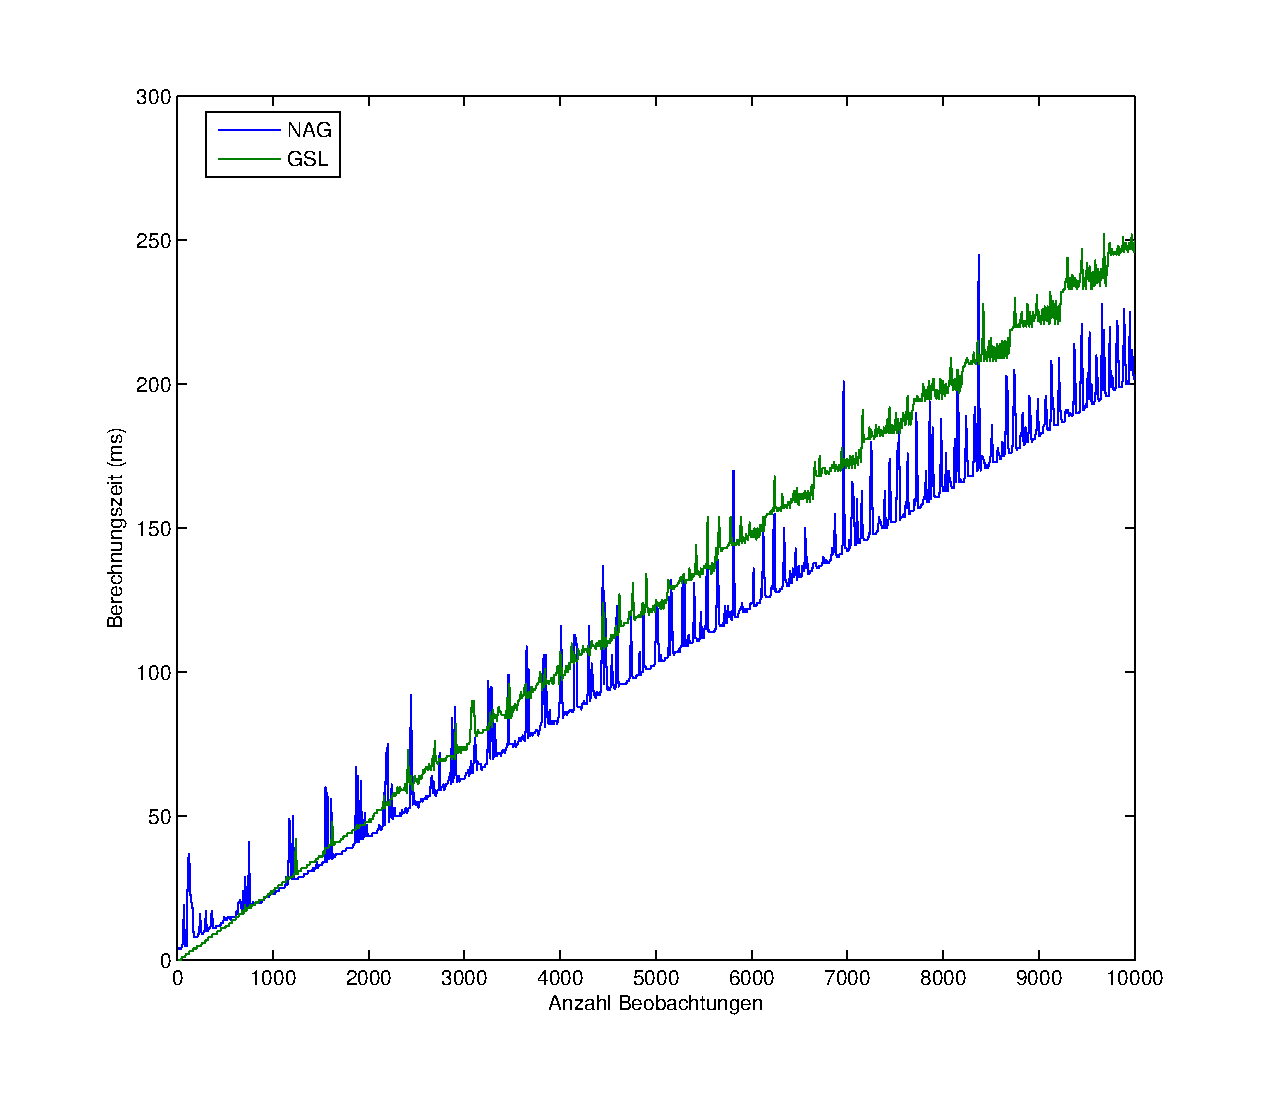
\includegraphics[width=0.6\textwidth]{figures/test_corr_1_random}
    }
    \subfloat[][Dauer der Berechnung des Bravais-Pearson-Korrelationskoeffizienten mit NAG und GSL (Münchener Mietspiegel 2003 \cite{Fahrmeir2011})]{
      \label{fig:analysis:test_corr_1_rent}
      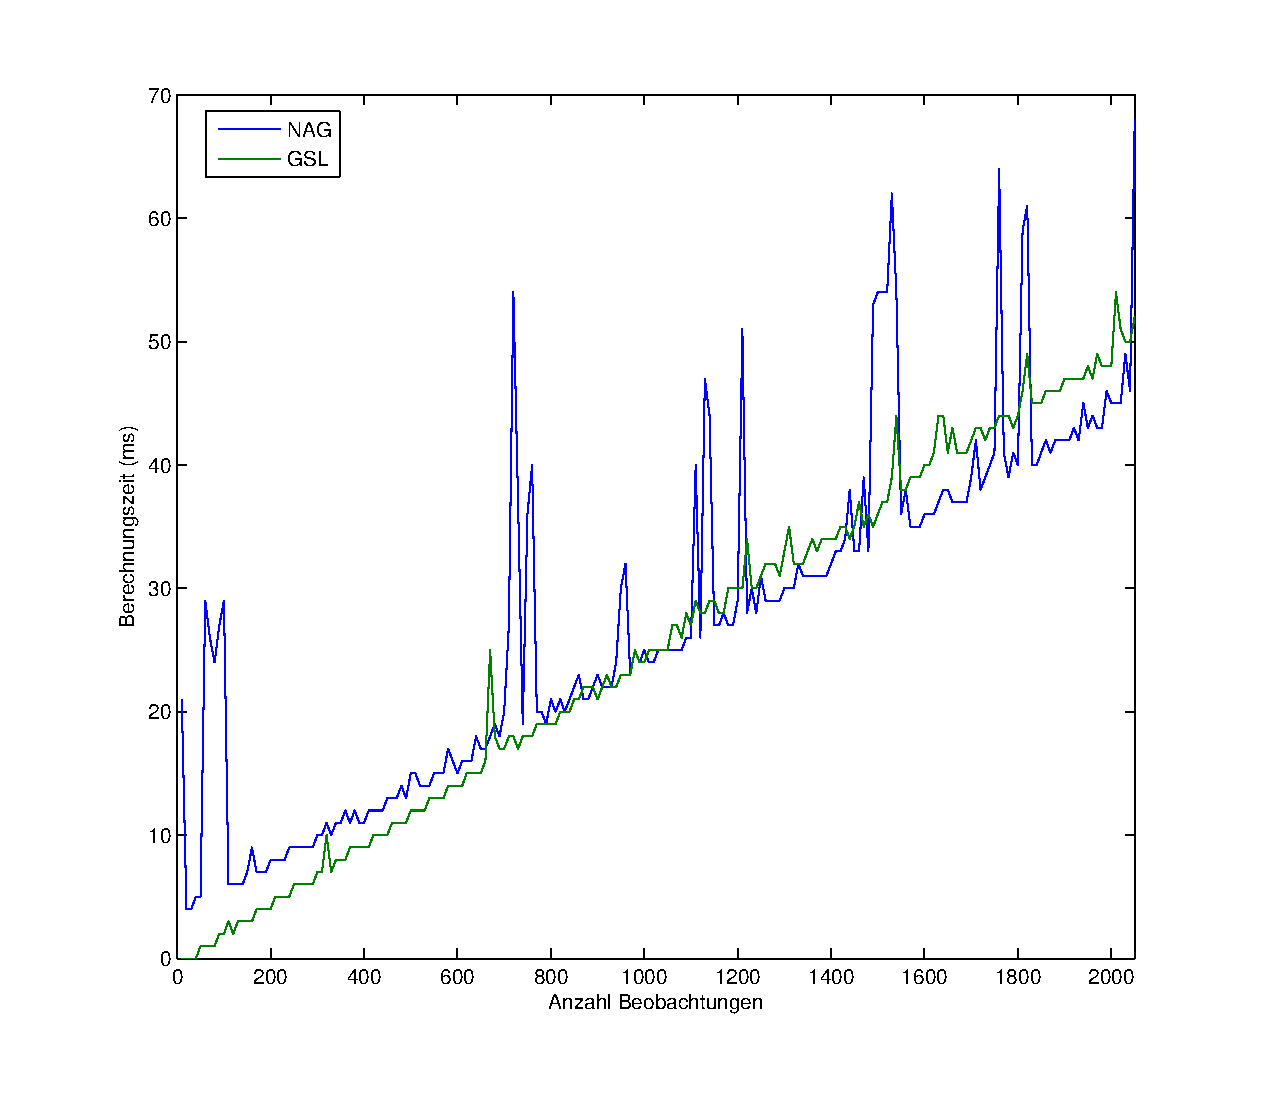
\includegraphics[width=0.6\textwidth]{figures/test_corr_1_rent}
    }\\
    \subfloat[][Dauer der Berechnung des Bravais-Pearson-Korrelationskoeffizienten und des Spearman-Rangkorrelationskoeffizienten mit NAG (Zufallsdatensatz)]{
      \label{fig:analysis:test_corr_2_random}
      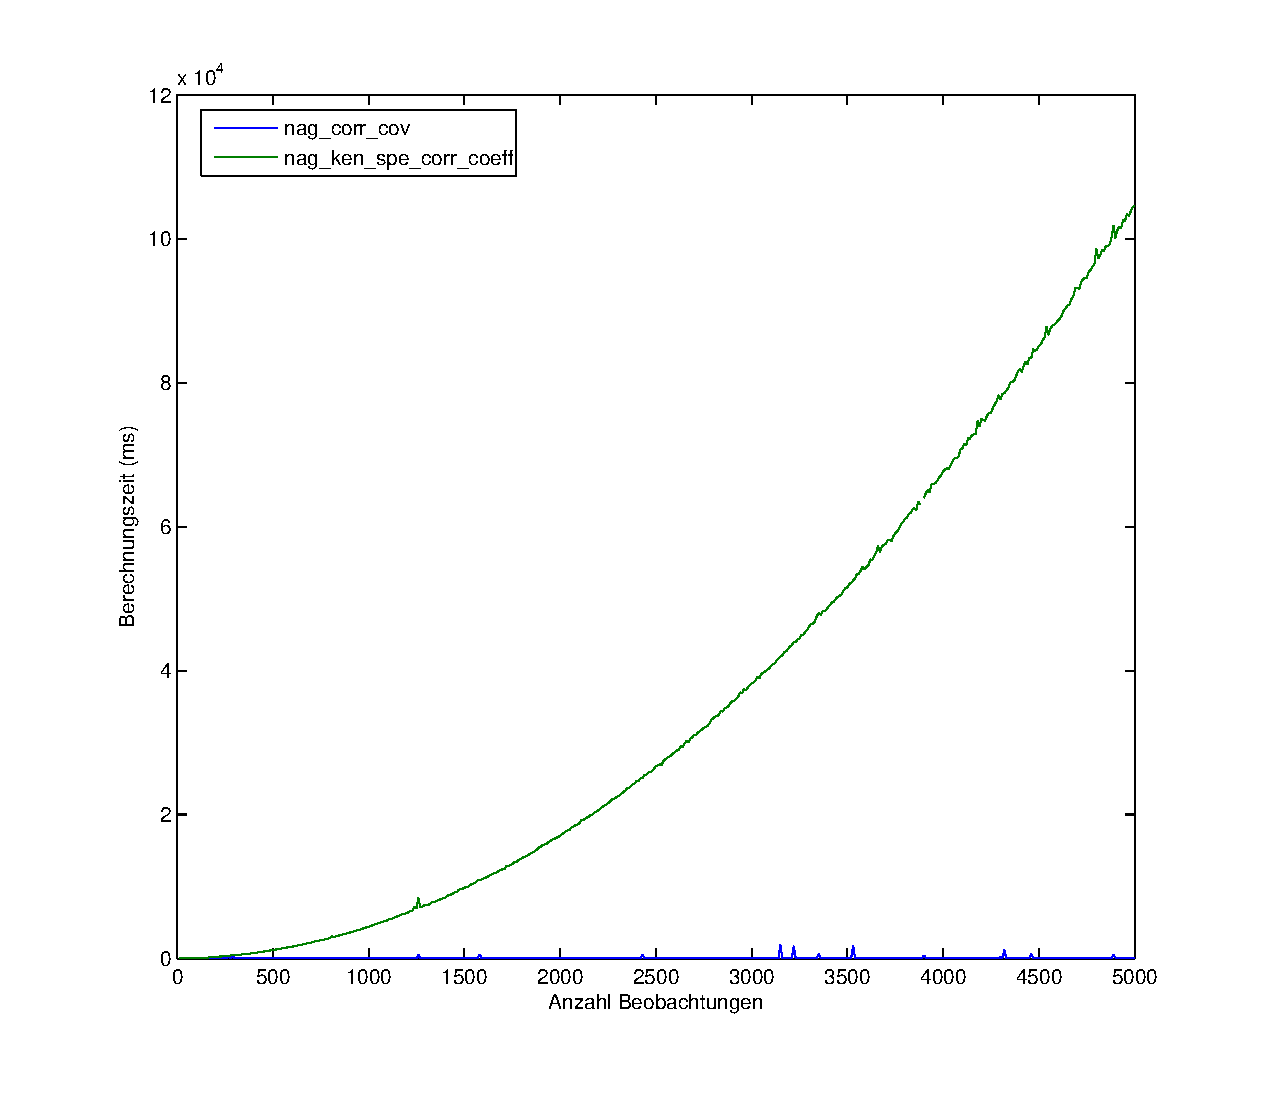
\includegraphics[width=0.6\textwidth]{figures/test_corr_2_random}
    }
    \subfloat[][Dauer der Berechnung des Bravais-Pearson-Korrelationskoeffizienten und des Spearman-Rangkorrelationskoeffizienten mit NAG (Münchener Mietspiegel 2003 \cite{Fahrmeir2011})]{
      \label{fig:analysis:test_corr_2_rent}
      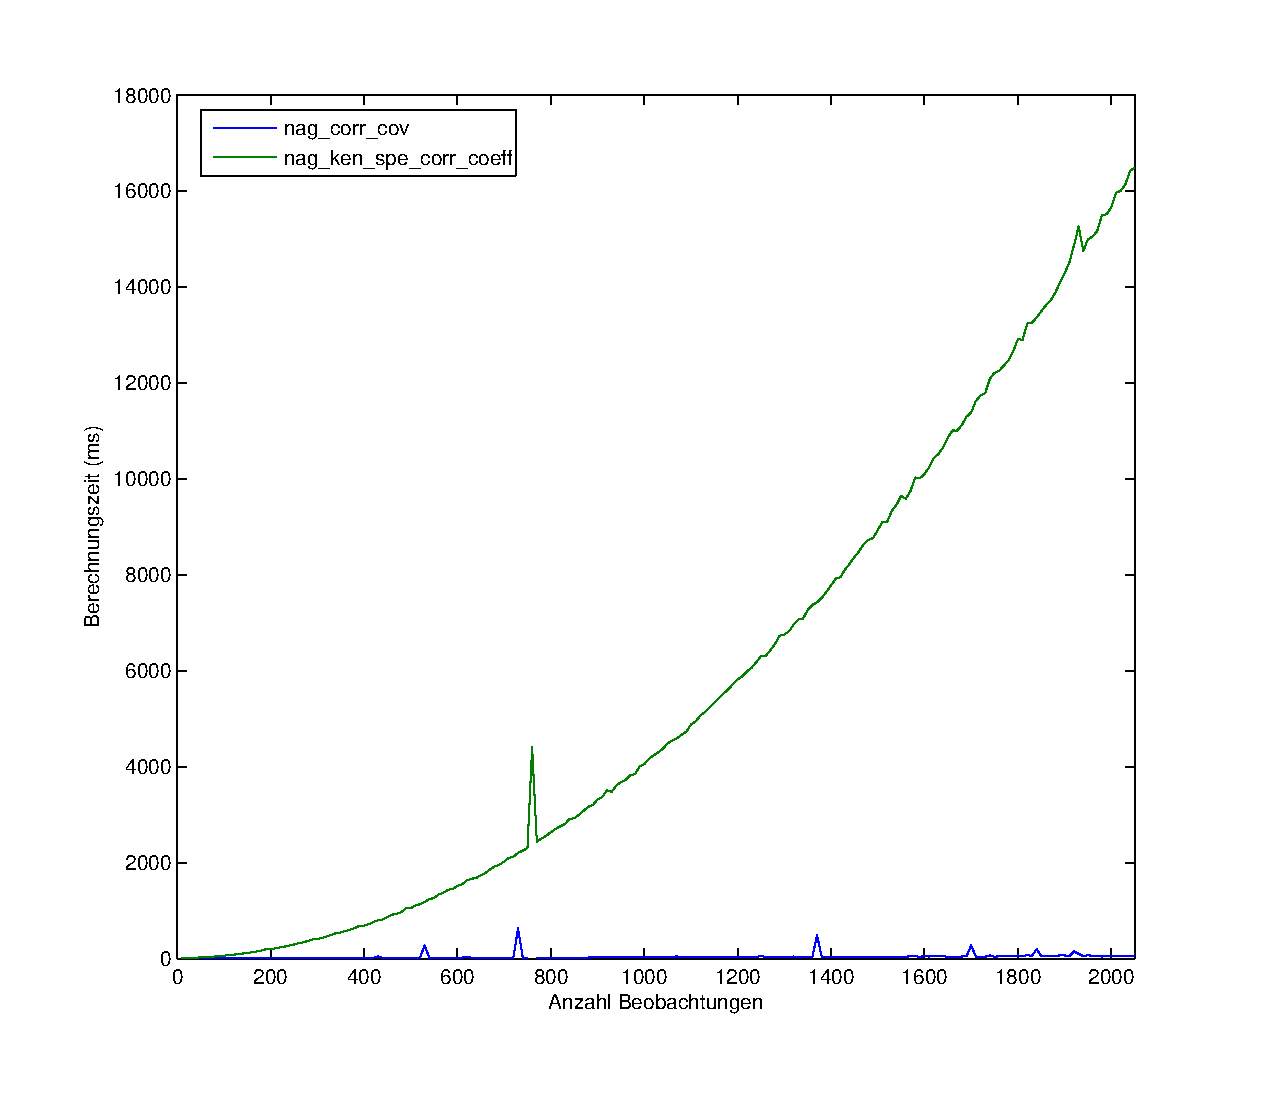
\includegraphics[width=0.6\textwidth]{figures/test_corr_2_rent}
    }\\
  \end{narrow}
  \caption{Ergebnisse der Leistungsanalyse zur Korrelation}
  \label{fig:analysis:correlation}
\end{figure}

% Graphik mit allen Kurven (Regression):
\begin{figure}[h]
  \centering
  \begin{narrow}{-0.2\textwidth}{0.2\textwidth}
    \subfloat[][Dauer der einfachen linearen Regression von NAG und GSL mit zunehmenden Beobachtungen aus dem Mietspiegeldatensatz\cite{Fahrmeir2011}.]{
      \label{fig:analysis:sim_reg_rent}
      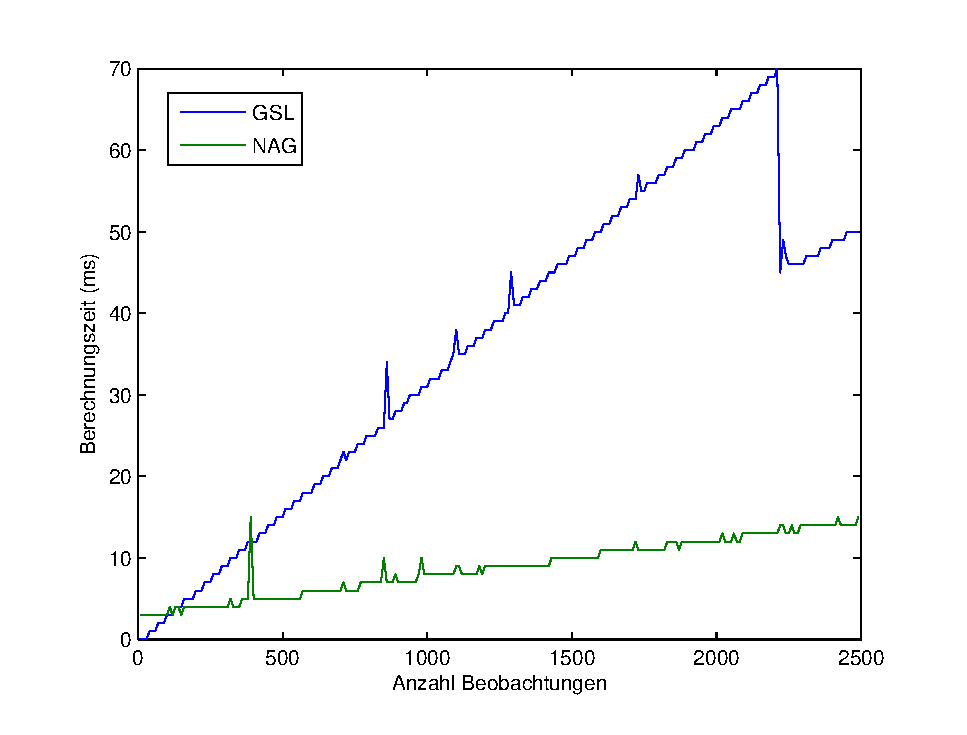
\includegraphics[width=0.6\textwidth]{figures/simple_reg_comp_rent}
    }
    \subfloat[][Dauer der einfachen linearen Regression von NAG und GSL mit zufälligen Daten.]{
      \label{fig:analysis:sim_reg_rand}
      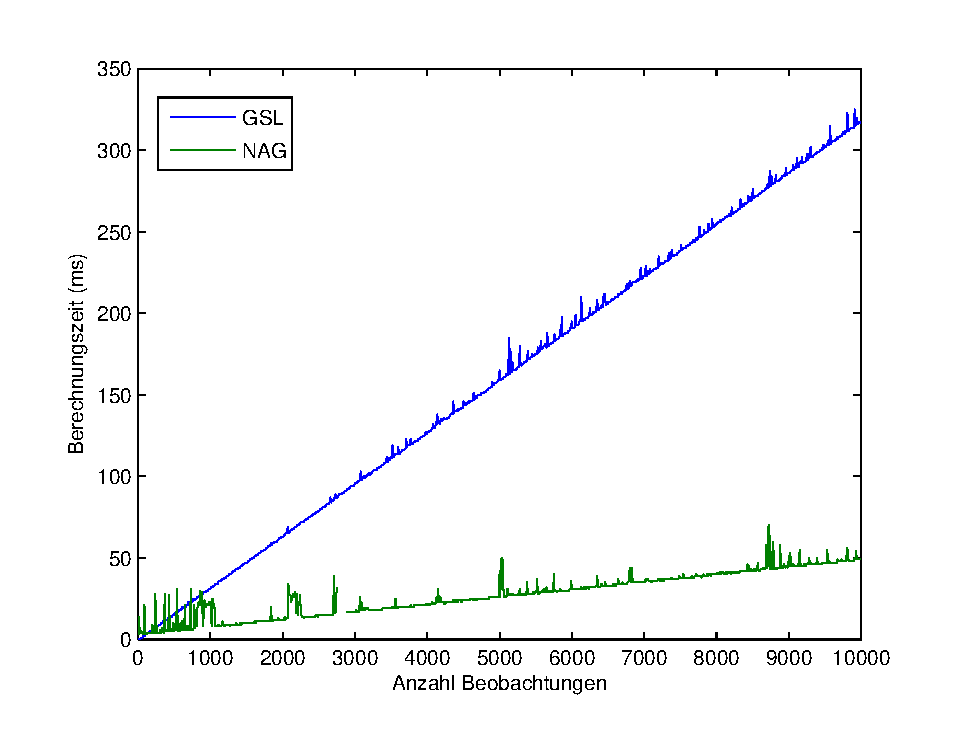
\includegraphics[width=0.6\textwidth]{figures/simple_reg_comp}
    }\\
    \subfloat[][Dauer der multiplen Regression von NAG und GSL mit 6 Merkmalen und zufälligen Daten.]{
      \label{fig:analysis:mul_reg_obs}
      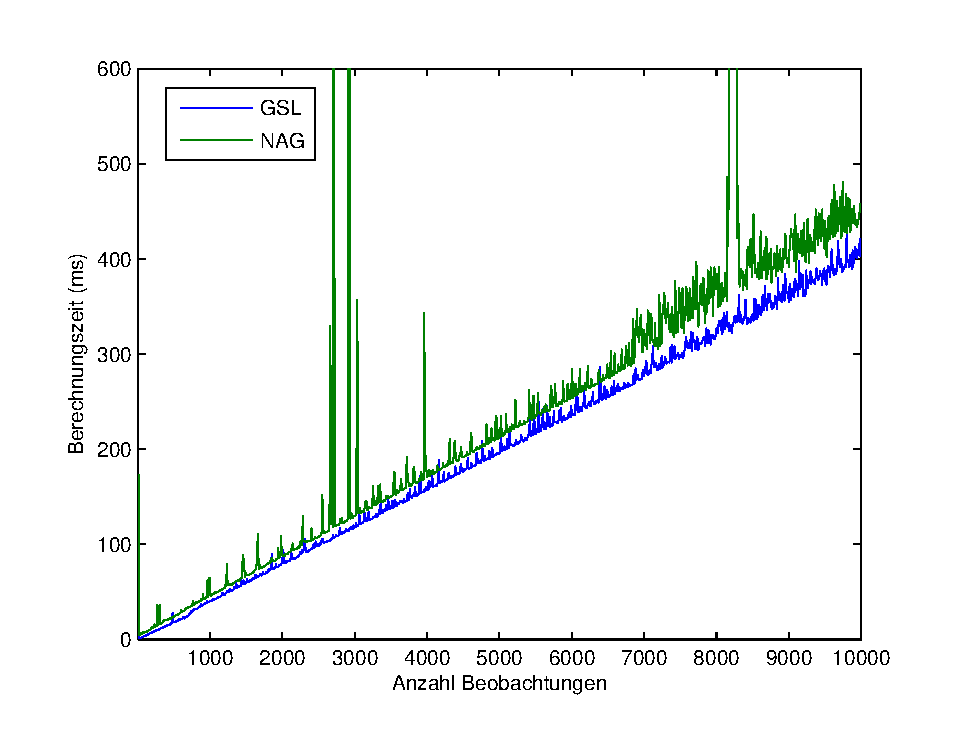
\includegraphics[width=0.6\textwidth]{figures/multi_reg_comp_6_var}
    }
    \subfloat[][Dauer der multiplen Regression von NAG und GSL mit 2500 Beobachtungen und zufälligen Daten.]{
      \label{fig:analysis:mul_reg_vars}
      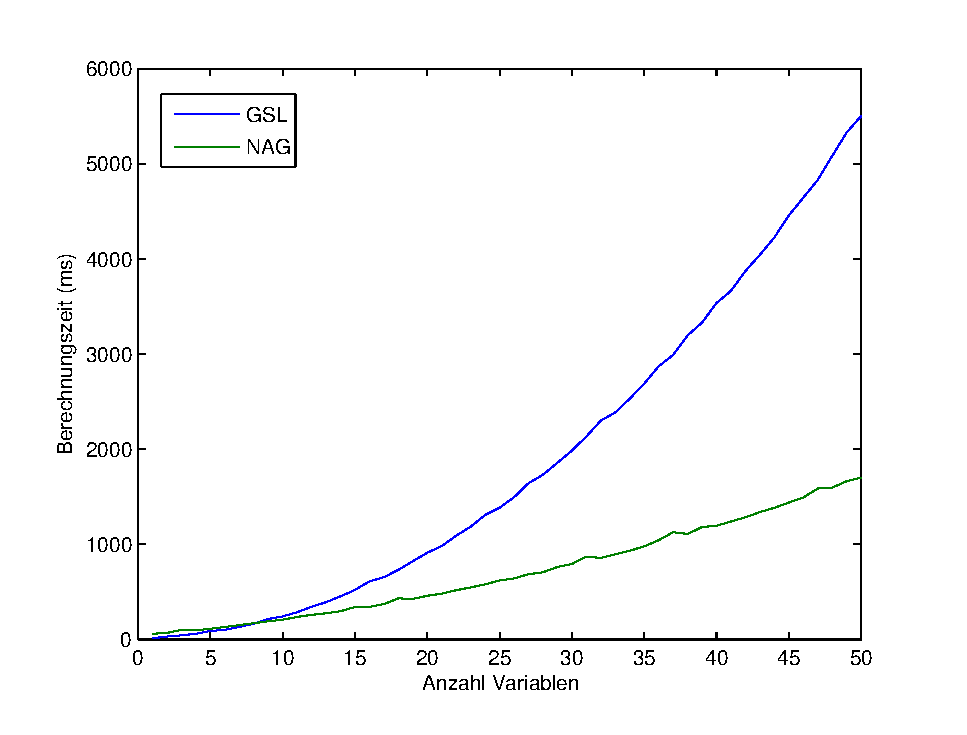
\includegraphics[width=0.6\textwidth]{figures/multi_reg_vars_2500_obs_rand}
    }\\
    \subfloat[][Unterschied zwischen direkter Berechnung und Aktualisierung mit Daten aus dem  Mietspiegeldatensatz\cite{Fahrmeir2011}.]{
      \label{fig:analysis:mul_reg_rent_act}
      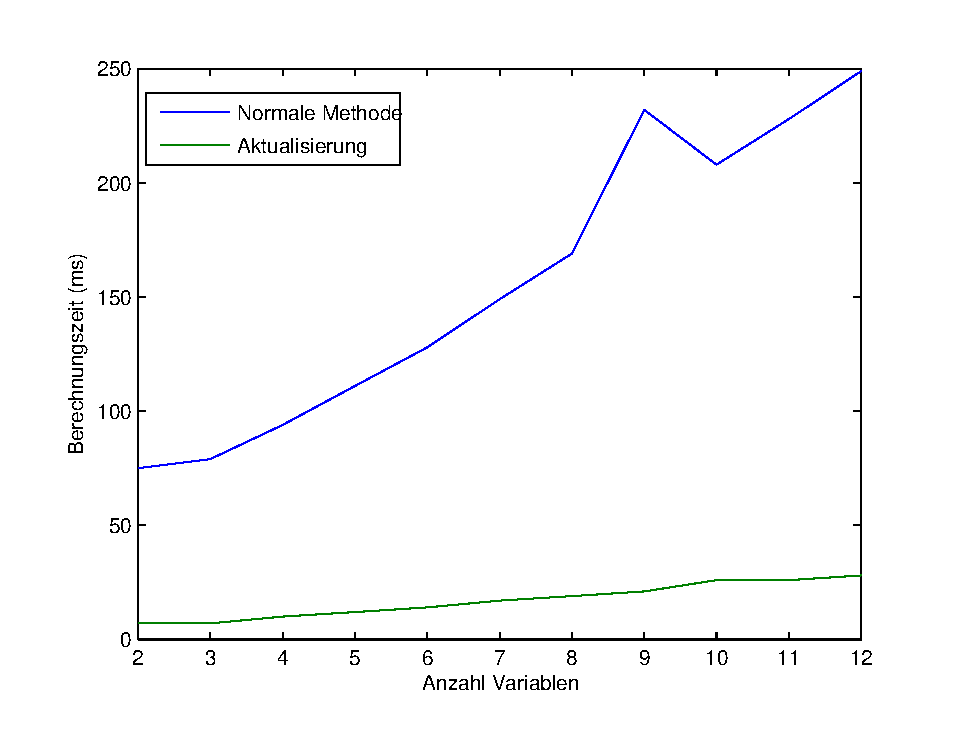
\includegraphics[width=0.6\textwidth]{figures/multi_reg_vars_2500_obs_act}
    }
    \subfloat[][Unterschied zwischen direkter Berechnung und Aktualisierung mit zufälligen Daten]{
      \label{fig:analysis:mul_reg_rand_act}
      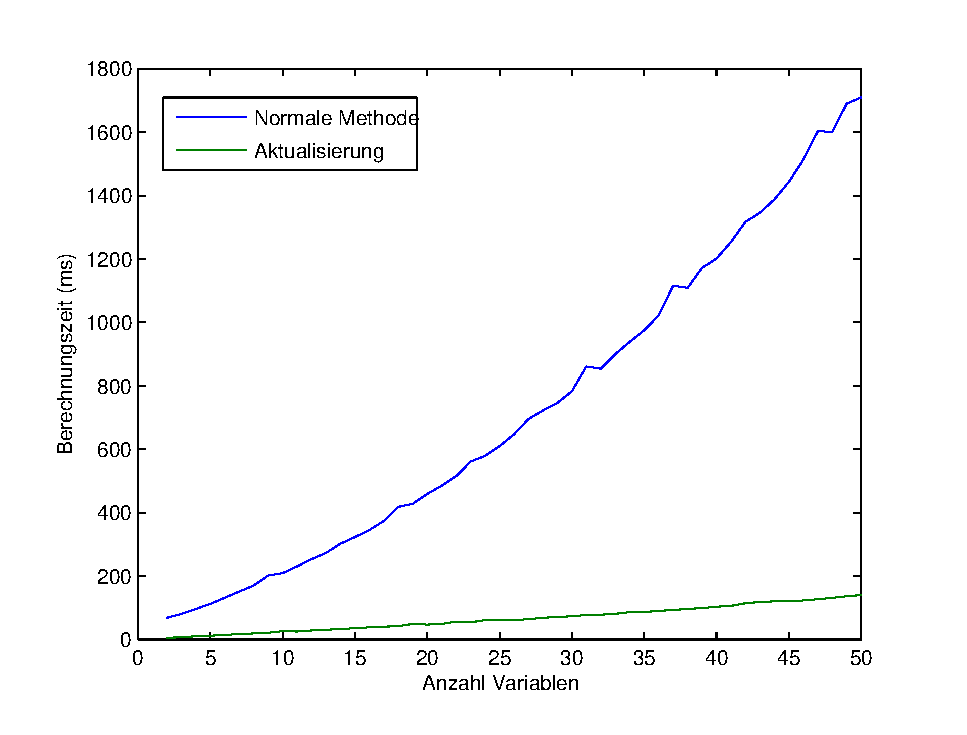
\includegraphics[width=0.6\textwidth]{figures/multi_reg_vars_2500_obs_act_rand}
    }
  \end{narrow}
  \caption{Ergebnisse der Leistungsanalyse zur Regression}
  \label{fig:analysis:regression}
\end{figure}

Hinsichtlich der Korrelation wurden zwei Tests durchgeführt: Im ersten Test wurde die {\it NAG}-Funktion zur Berechnung des Korrelationskoeffizienten nach Bravais und Pearson ({\it nag\_corr\_cov}) mit ihrem {\it GSL}-Pendant ({\it gsl\_stats\_correlation}) verglichen. Im zweiten Test wurden innerhalb der\naglib die Funktion zur Berechnung des Korrelationskoeffizienten nach Bravais und Pearson sowie jene zur Berechnung des Rangkorrelationskoeffizienten nach Spearman verglichen.

Der Testaufbau war in beiden Fällen gleich: Die verglichenen Funktionen erhielten pro Durchgang als Eingabe jeweils zwei Merkmale aus einem Zufallsdatensatz sowie anschließend aus dem {\it Münchener Mietspiegel 2003} \cite{Fahrmeir2011}. Während eines Durchgangs wurde die Anzahl der Beobachtungen schrittweise von 10 auf 10000 (Zufallsdatensatz) bzw. 2050 ({\it Münchener Mietspiegel 2003}) erhöht. Die Schrittweite betrug dabei 10. In jedem Schritt wurde die jeweilige Funktion 1000 mal berechnet und die gesamte Berechnungszeit gemessen.

Die Ergebnisse des ersten Tests sind in \reffig{fig:analysis:test_corr_1_random} und \reffig{fig:analysis:test_corr_1_rent} zu sehen. Wie gut ersichtlich ist, zeigen beide Funktionen ein lineares Wachstum, wobei die Berechnungszeit der {\it GSL}-Funktion bis zu etwa 900 Beobachtungen geringer als die der {\it NAG}-Funktion ist. Diese zeigt sich jedoch für jede größere Anzahl Beobachtungen im Durchschnitt (d.h. unter Relativierung der sichtbaren Schwankungen der Berechnungszeit) als geeigneter: Bei einer Anzahl von 10000 Beobachtungen braucht sie bereits etwa 45 ms weniger. Eine Empfehlung zur Verwendung der beiden Funktionen könnte daher lauten, erstere nur für kleine Datensätze zu verwenden und letztere für größere Datensätze ab etwa 900 Beobachtungen. Insgesamt hat hier also die {\it NAG}-Funktion die Nase vorn.

Die Ergebnisse des zweiten Tests können in \reffig{fig:analysis:test_corr_1_random} und \reffig{fig:analysis:test_corr_1_rent} abgelesen werden. Hier ist deutlich erkennbar, dass die Funktion zur Berechnung des Korrelationskoeffizienten nach Bravais und Pearson wesentlich schneller ist als jene zur Berechnung des Rangkorrelationskoeffizienten nach Spearman. Dies ist vermutlich durch die Berechnung der Ränge zu erklären, welche letztere Funktion zusätzlich leisten muss: Wenn man bedenkt, dass zur Rangbildung alle Beobachtungen zuerst nach ihren Messwerten sortiert werden müssen (siehe \refsec{sec:spear_rangkorr}) und es bekanntermaßen bisher keinen Sortieralgorithmus mit einer Worst-Case-Laufzeit von weniger als $\mathcal{O}(n \log{n})$ gibt. Eine Empfehlung ist daher, letztere Funktion wirklich nur dann einzusetzen, wenn sie zur Berechnung der Korrelation von ordinalskalierten Merkmalen unbedingt benötigt wird.

Für die Regression werden jeweils die Funktionen für die einfache und multiple lineare Regression der \naglib mit den Funktionen der GSL verglichen.
In Abbildung \ref{fig:analysis:sim_reg_rent} sind die Berechnungszeiten der Funktionen nag\_simple\_linear\_"-regression und gsl\_fit\_linear bei steigender Beobachtungszahl und unter Benutzung der Daten des Münchener Mietspiegels gezeigt.
Die angegebenen Zeiten entsprechen dabei jeweils 1000 Berechnungen.
Es ist zu erkennen, dass die NAG Funktion weit besser skaliert und bei 2500 Beobachtungen um den Faktor 3-4 schneller ist.
Dabei ist aber zu berücksichtigen, dass bei der NAG Funktion zusätzlich zum Regressionskoeffizienten und der Quadratsumme der Residuen noch und das Bestimmtheitsmaß und den Standardfehler berechnet, während die GSL Funktion zusätzlich die Kovarianzen der Koeffizienten zurück gibt.
Der Einbruch der Berechnungszeiten bei 2200 Beobachtungen ist reproduzierbar und tritt nur bei diesem Datensatz auf.
Der erkennbare Trend wird durch einen Vergleich mit zufälligen Daten und mehr Beobachtungen noch verstärkt (vgl. Abbildung \ref{fig:analysis:sim_reg_rand}).

Für den Vergleich der Leistungsfähigkeit bei der Berechnung der multiplen linearen Regression wurden zwei verschiedene Setups gewählt.
Zum einen wird wieder sukzessive die Anzahl der Beobachtungen erhöht zum anderen ist die Zahl der Regressoren variabel. 
Für beide Ansätze werden zufällige Daten benutzt, da die Anzahl der Beobachtungen und der Variablen hier nicht limitiert sind.
% TODO: Nummer des Anhangs einfügen
Da die Funktionen, wie auch bei der einfachen Regression, wieder nicht die gleichen Resultate zurück liefern, wurde bei der GSL Funktion zusätzlich das Bestimmtheitsmaß und die Residuen berechnet, um einigermaßen vergleichbare Daten zu erhalten (siehe Anhang ??).
Die Ergebnisse bei variablen Beobachtungen und sechs Regressoren sind in Abbildung \ref{fig:analysis:mul_reg_obs} zu sehen.
Die beiden Bibliotheken liegen hier fast gleichauf, wobei sich leichte Vorteile für die GSL zeigen.
Abbildung \ref{fig:analysis:mul_reg_vars} zeigt die Ergebnisse bei einer steigender Anzahl an Variablen bei 2500 Beobachtungen.
Auch hier liegt die GSL bei wenigen Regressoren vorne, ab neun Regressoren ist allerdings die NAG Funktion effizienter, welche auch bei weiter steigender Regressorenzahl besser skaliert.
Natürlich ist dabei zu bedenken, dass in den meisten Anwendungen wahrscheinlich nicht mehr als zehn Regressoren verwendet werden.

Außerdem haben wir noch die Geschwindigkeit der Methoden zur Aktualisierung eines Modells mit der der Neuberechnung in der \naglib verglichen.
Als veränderbaren Faktor benutzen wir hier wieder die Anzahl der Regressoren bei 100 Iterationen.
Es ist sowohl bei der Verwendung der Mietdaten (Abbildung \ref{fig:analysis:mul_reg_rent_act}), als auch bei der Verwendung von zufälligen Daten (Abbildung \ref{fig:analysis:mul_reg_rand_act}) zu erkennen, dass die Aktualisierungsmethode besser skaliert und um eine Faktor von 8 oder mehr schneller ist.
Dabei muss allerdings, wie schon zuvor erwähnt, berücksichtigt werden, dass die Regressionsergebnisse nicht äquivalent sind.

%%% Local Variables: 
%%% mode: latex
%%% TeX-master: "report"
%%% End: 

%  LocalWords:  GSL Konfidenzintervalle Leistungsanalyse Quadratsumme
%  LocalWords:  Berechnungszeiten Beobachtungszahl Standardfehler
